\section{Reprezentacja dyskretnej zmiennej ciągłej}
\begin{frame}{Reprezentacja dyskretnej zmiennej ciągłej - zmienna}

	
	\begin{minipage}{0.6\textwidth}\raggedright
		x - ciągła zmienna niezależna \\
        $X_{1} \leq x \leq X_{2}$ \\ 
        $\newline \newline$
        siatka(przestrzenna) punktów: \\
        $1 \leq j \leq J \rightarrow \textrm{węzły siatki}$ \\
        $\Delta x_{j}$ - kroki siatki
        \\
        $\newline \newline$
        $x \rightarrow \{ x_{j} \}$ \\
        zmienna ciągła $\rightarrow$ wektor o wymierze J
        
	\end{minipage}
    \hfill%
    \begin{minipage}{0.385\textwidth}
		%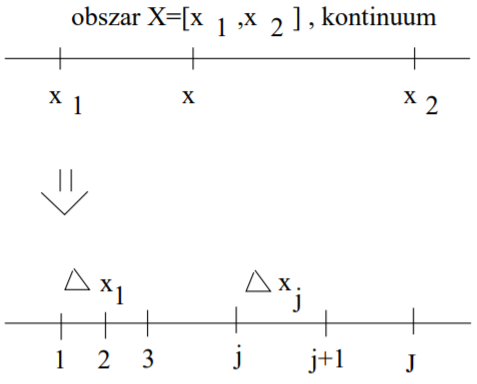
\includegraphics[width=\linewidth]{img/20/mrs_img_1}
        \begin{figure}[t]
			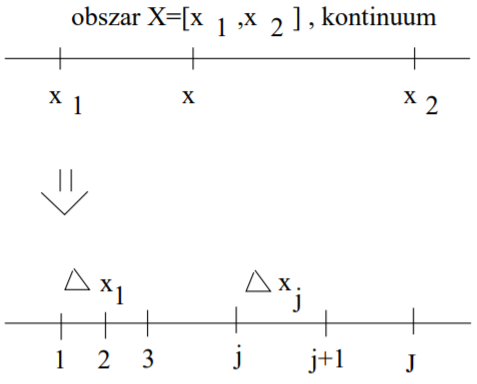
\includegraphics[width=5cm]{img/20/mrs_img_1}
		\end{figure}
	\end{minipage}%
	
\end{frame}
%%%%%%%%%%%%%%%%%%5
\begin{frame}{c.d. - funkcja}
	\[
    	\underbrace{f(x)}_{\substack{\textrm{funkcja określona} \\ 
        \textrm{na kontinuum}}}
        = \underbrace{\{ f_{j}=j(x_{j}) \}}
        _{\substack{\textrm{wektor określony} \\ 
        \textrm{na siatce} \  \{ x_{j} \} }}
    \]
    W dowolnym $x': \ x_{j} \leq x' \leq x_{j+1} \newline$
    $f(x)$ można przybliżyć stosując interpolacje liniową:
    \[
    	\epsilon = \frac{x' - x_{j}}{x_{j+1}-x_{j}}
    \]
    \[
    	f^{*} = \epsilon \cdot f_{j+1} + (1- \epsilon) \cdot f_{j}
    \]
\end{frame}














